\documentclass{ximera}

%\documentclass{ximera}

\usepackage{float}
\usepackage{subcaption}

\pgfplotsset{compat=1.16}

\newtheorem{ass}{Assumption}

\def\check{\tikz\fill[scale=0.4](0,.35) -- (.25,0) -- (1,.7) -- (.25,.15) -- cycle;}





\outcome{Use parity to establish important equalities.}

\author{Brad Waller}

%Section 2.4

\title{Parity}

\begin{document}

\begin{abstract}
Our no arbitrage and frictionless transaction assumptions have some hefty implications, many of which are explored here.
\end{abstract}

\maketitle
In the last few sections, we have developed the notion of options, a special type of derivative. These are the derivatives that much of this text will work with. With these derivatives come some special relationships that follow from our no arbitrage assumption and the further assumption of frictionless markets (that is, no fees on transactions). The simplest relationship comes from comparing our cash-or-nothing options. Recall our diagram for these options.

\begin{center}
	\begin{tikzpicture}[scale=0.7]
	\begin{axis}[
		xmin=0,
		xmax=45,
		%xtick={5,10,...,50},
		ymin=-2,
		ymax=3,
		%ytick={-20,-10,...,50},
		%grid=both,
		axis lines=middle,
		axis line style={->, >=latex},
		x label style={at={(0.95,0.42)}},
		%x label style={at={(axis description cs:0.86,0.42)},anchor=north},
		xlabel={$S(T)$},
		ylabel={payoff}]
		%style={font=\tiny}]
		\addplot[black, smooth, domain=0:25, -, >=latex]{1};
	\end{axis}
	\node at (3.5, -0.2){\small C/N Put Payoff};
	\end{tikzpicture}
	\hspace{10pt}
	\begin{tikzpicture}[scale=0.7]
	\begin{axis}[
		xmin=0,
		xmax=45,
		%xtick={5,10,...,50},
		ymin=-2,
		ymax=3,
		%ytick={-20,-10,...,50},
		%grid=both,
		axis lines=middle,
		axis line style={->, >=latex},
		x label style={at={(0.95,0.42)}},
		xlabel={$S(T)$},
		ylabel={payoff}]
		%style={font=\tiny}]
		\addplot[black, smooth, domain=25:42, ->, >=latex]{1};
	\end{axis}
	\node at (3.5,-0.2){\small C/N Call Payoff};
	\end{tikzpicture}
\end{center}

If we were lazy and drew these both on one graph, we would have the following:

\begin{center}
	\begin{tikzpicture}[scale=0.7]
	\begin{axis}[
		xmin=0,
		xmax=45,
		%xtick={5,10,...,50},
		ymin=-2,
		ymax=3,
		%ytick={-20,-10,...,50},
		%grid=both,
		axis lines=middle,
		axis line style={->, >=latex},
		x label style={at={(0.95,0.42)}},
		%x label style={at={(axis description cs:0.86,0.42)},anchor=north},
		xlabel={$S(T)$},
		ylabel={payoff}]
		%style={font=\tiny}]
		\addplot[black, smooth, domain=0:42, ->, >=latex]{1};
	\end{axis}
	\end{tikzpicture}
\end{center}

That's actually quite revealing. What this says is that the position of owning a cash-or-nothing put and cash-or-nothing call is equivalent to \$1 at time $T$! We should all know that the price of the position of \$1 at time $T$ is simply its present value. Without knowing anything more, we have
\begin{equation}
c_{C/N}+p_{C/N}=e^{rT}.
\end{equation}
In words, the price of the portfolio consisting of a cash-or-nothing put and cash-or-nothing call is the present value of one dollar. This is all under the assumption that the put and call have the same underlying asset, same strike, expiration at time $T$, and are European. This is particularly wonderful since we have no idea how much our options cost on their own! Let's see if we can do something similar with asset-or-nothing options.

\begin{center}
	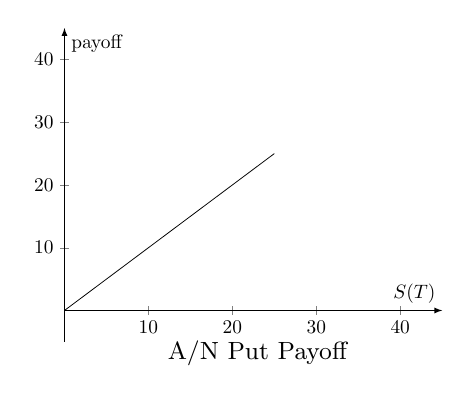
\begin{tikzpicture}[scale=0.7]
	\begin{axis}[
		xmin=0,
		xmax=45,
		%xtick={5,10,...,50},
		ymin=-5,
		ymax=45,
		%ytick={-20,-10,...,50},
		%grid=both,
		axis lines=middle,
		axis line style={->, >=latex},
		%x label style={at={(0.9,0.05)}},
		%x label style={at={(axis description cs:0.86,0.42)},anchor=north},
		xlabel={$S(T)$},
		ylabel={payoff}]
		%style={font=\tiny}]
		\addplot[black, smooth, domain=0:25, -, >=latex]{x};
	\end{axis}
	\node at (3.5, -0.2){\small A/N Put Payoff};
	\end{tikzpicture}
	\hspace{10pt}
	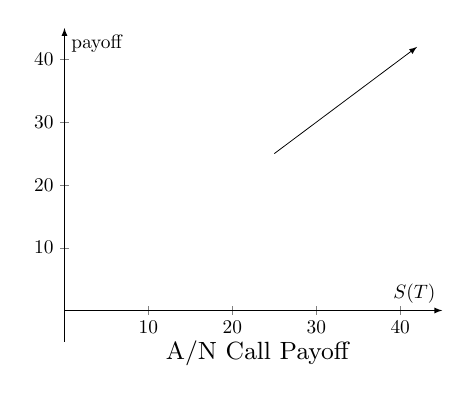
\begin{tikzpicture}[scale=0.7]
	\begin{axis}[
		xmin=0,
		xmax=45,
		%xtick={5,10,...,50},
		ymin=-5,
		ymax=45,
		%ytick={-20,-10,...,50},
		%grid=both,
		axis lines=middle,
		axis line style={->, >=latex},
		%x label style={at={(axis description cs:0.86,0.42)},anchor=north},
		xlabel={$S(T)$},
		ylabel={payoff}]
		%style={font=\tiny}]
		\addplot[black, smooth, domain=25:42, ->, >=latex]{x};
	\end{axis}
	\node at (3.5, -0.2){\small A/N Call Payoff};
	\end{tikzpicture}
\end{center}

Let's be lazy once again!

\begin{center}
	\begin{tikzpicture}[scale=0.7]
	\begin{axis}[
		xmin=0,
		xmax=45,
		%xtick={5,10,...,50},
		ymin=-5,
		ymax=45,
		%ytick={-20,-10,...,50},
		%grid=both,
		axis lines=middle,
		axis line style={->, >=latex},
		%x label style={at={(axis description cs:0.86,0.42)},anchor=north},
		xlabel={$S(T)$},
		ylabel={payoff}]
		%style={font=\tiny}]
		\addplot[black, smooth, domain=0:42, ->, >=latex]{x};
	\end{axis}
	\end{tikzpicture}
\end{center}

This laziness is really working out! The picture here is quite revealing as well. It shows that the portfolio consisting of an asset-or-nothing put and an asset-or-nothing call will pay just like the underlying asset itself at time $T$. The bad news is that it's a little bit more difficult to price this position; however, if we recall there is a special value we can pay today to guarantee this payoff. Try to think what it is before you read the next sentence. It is the prepaid forward price for the underlying asset. We have
\begin{equation}
c_{A/N}+p_{A/N}=S(0)e^{-\delta T}.
\end{equation}
In words, the price of the portfolio consisting of a asset-or-nothing put and asset-or-nothing call is the prepaid forward price of the underlying asset. This is all under the assumption that the put and call have the same underlying asset, same strike, expiration at time $T$, and are European. Everything is going rather well. Let's try something similar to our regular calls and puts. 

\begin{center}
	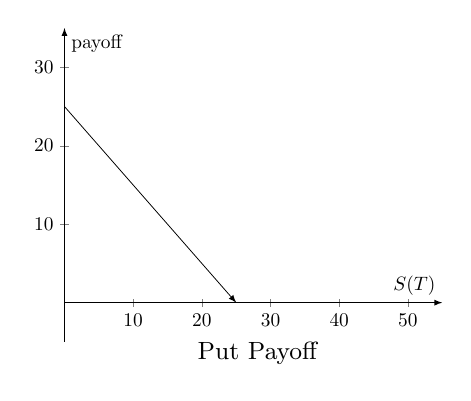
\begin{tikzpicture}[scale=0.7]
	\begin{axis}[
		xmin=0,
		xmax=55,
		%xtick={5,10,...,50},
		ymin=-5,
		ymax=35,
		%ytick={-20,-10,...,50},
		%grid=both,
		axis lines=middle,
		axis line style={->, >=latex},
		%x label style={at={(0.9,0.05)}},
		%x label style={at={(axis description cs:0.86,0.42)},anchor=north},
		xlabel={$S(T)$},
		ylabel={payoff}]
		%style={font=\tiny}]
		\addplot[black, smooth, domain=0:25, ->, >=latex]{25-x};
	\end{axis}
	\node at (3.5, -0.2){\small Put Payoff};
	\end{tikzpicture}
	\hspace{10pt}
	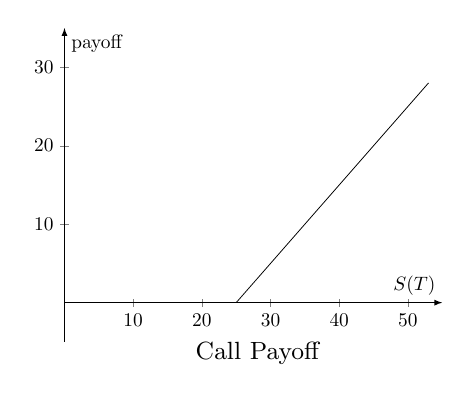
\begin{tikzpicture}[scale=0.7]
	\begin{axis}[
		xmin=0,
		xmax=55,
		%xtick={5,10,...,50},
		ymin=-5,
		ymax=35,
		%ytick={-20,-10,...,50},
		%grid=both,
		axis lines=middle,
		axis line style={->, >=latex},
		%x label style={at={(axis description cs:0.86,0.42)},anchor=north},
		xlabel={$S(T)$},
		ylabel={payoff}]
		%style={font=\tiny}]
		\addplot[black, smooth, domain=25:53, -, >=latex]{x-25};
	\end{axis}
	\node at (3.5, -0.2){\small Call Payoff};
	\end{tikzpicture}
\end{center}

Letting laziness strike, we have

\begin{center}
	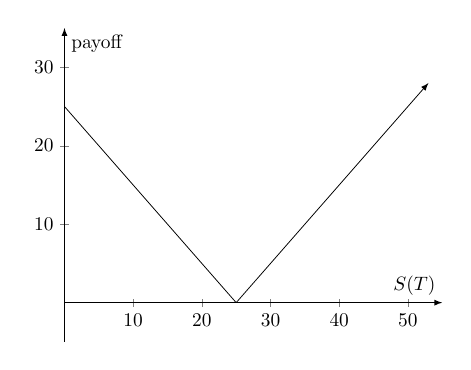
\begin{tikzpicture}[scale=0.7]
	\begin{axis}[
		xmin=0,
		xmax=55,
		%xtick={5,10,...,50},
		ymin=-5,
		ymax=35,
		%ytick={-20,-10,...,50},
		%grid=both,
		axis lines=middle,
		axis line style={->, >=latex},
		%x label style={at={(axis description cs:0.86,0.42)},anchor=north},
		xlabel={$S(T)$},
		ylabel={payoff}]
		%style={font=\tiny}]
		\addplot[black, smooth, domain=0:25, -, >=latex]{25-x};
		\addplot[black, smooth, domain=25:53, ->, >=latex]{x-25};
	\end{axis}
	\end{tikzpicture}
\end{center}

Hmmm... that didn't do what I had hoped. Perhaps if I write the put instead.

\begin{center}
	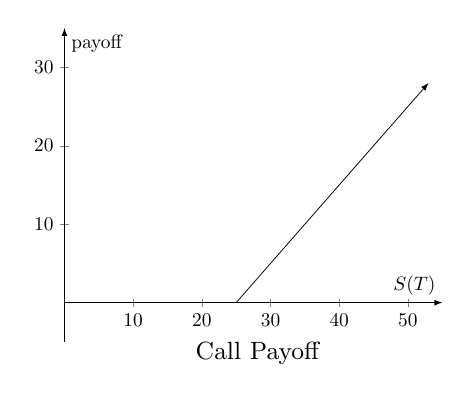
\begin{tikzpicture}[scale=0.7]
	\begin{axis}[
		xmin=0,
		xmax=55,
		%xtick={5,10,...,50},
		ymin=-5,
		ymax=35,
		%ytick={-20,-10,...,50},
		%grid=both,
		axis lines=middle,
		axis line style={->, >=latex},
		%x label style={at={(0.9,0.05)}},
		%x label style={at={(axis description cs:0.86,0.42)},anchor=north},
		xlabel={$S(T)$},
		ylabel={payoff}]
		%style={font=\tiny}]
		\addplot[black, smooth, domain=25:53, ->, >=latex]{x-25};
	\end{axis}
	\node at (3.5, -0.2){\small Call Payoff};
	\end{tikzpicture}
	\hspace{10pt}
	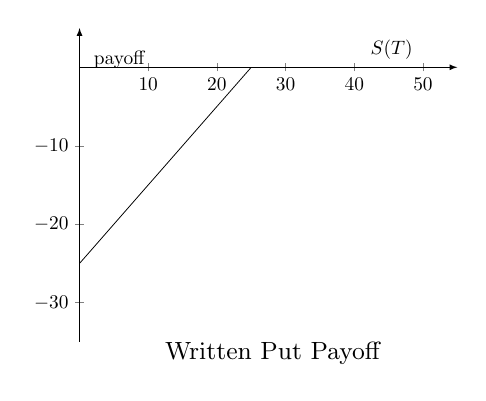
\begin{tikzpicture}[scale=0.7]
	\begin{axis}[
		xmin=0,
		xmax=55,
		%xtick={5,10,...,50},
		ymin=-35,
		ymax=5,
		%ytick={-20,-10,...,50},
		%grid=both,
		axis lines=middle,
		axis line style={->, >=latex},
		x label style={at={(0.9, 0.88)}},
		y label style={at={(0.02, 0.95)}},
		xlabel={$S(T)$},
		ylabel={payoff}]
		%style={font=\tiny}]
		\addplot[black, smooth, domain=0:25, -, >=latex]{x-25};
	\end{axis}
	\node at (3.5, -0.2){\small Written Put Payoff};
	\end{tikzpicture}
\end{center}

Unleash the lazy!

\begin{center}
	\begin{tikzpicture}[scale=0.7]
	\begin{axis}[
		xmin=0,
		xmax=55,
		%xtick={5,10,...,50},
		ymin=-35,
		ymax=35,
		%ytick={-20,-10,...,50},
		%grid=both,
		axis lines=middle,
		axis line style={->, >=latex},
		x label style={at={(0.9, 0.55)}},
		xlabel={$S(T)$},
		ylabel={payoff}]
		%style={font=\tiny}]
		\addplot[black, smooth, domain=0:53, ->, >=latex]{x-25};
	\end{axis}
	\end{tikzpicture}
\end{center}

That certainly looks better. There's a few ways to think of this. I think the most direct is that the position of ownership in a call and a written put is equivalent to a position that pays $S(T)-K$ at time $T$. Fortunately, we have a derivative that does just that: a forward contract. This yields
\begin{equation}
c-p=S(0)e^{-\delta T}-Ke^{-rT}.
\end{equation}
In words, since a call and a written put have the same payoff of the forward contract, it must be the case that the portfolio consisting of the call and written put has equivalent value to the forward contract. All derivatives in this arrangement have the same expiration and same underlying asset. In addition, the strikes of the options are the same as the agreed upon price in the forward contract. Finally, the options must all be European. 

We can combine these equations into the following theorem.

\begin{theorem}[Parity]
The equations numbered in this section are given special names due to their importance. In order they are {\bf cash-or-nothing parity}
	\begin{equation*}
	c_{C/N}+p_{C/N}=e^{-rT},
	\end{equation*}
{\bf asset-or-nothing parity}
	\begin{equation*}
	c_{A/N}+p_{A/N}=S(0)e^{-\delta T},
	\end{equation*}
and {\bf put-call-parity}
	\begin{equation*}
	c-p=S(0)e^{-\delta T}-Ke^{-rT}.
	\end{equation*}
In each equation, the derivatives must all have the same terms. 
\end{theorem}

\begin{remark}
These are not all the possibilities for parity. This is simply a glimpse into how parity relationships work. For example, an alternative to put call parity would be to say that the position consisting of a call and a written put is equivalent to purchasing $e^{-\delta T}$ shares of the underlying asset and selling (or issuing) $Ke^{-rT}$ in bonds today. 
\end{remark}

Since the cash-or-nothing options don't have the most exciting arbitrage opportunities, let's work with an asset-or-nothing option.

\begin{example}
You are given the price of two asset-or-nothing options: $c_{A/N}=31.97$ and $p_{A/N}=34.08$. Both options have the same underlying asset, the same strike and the same time to expiration (three months from today). The asset costs $70$ today and has a dividend rate of $2\%$. Determine if there is an arbitrage opportunity.
\end{example}

\begin{solution}
We only have one test for this condition: asset-or-nothing parity. We must verify that the equality holds. If it doesn't, then we have the recipe for arbitrage.
	\begin{align*}
	c_{A/N}+p_{A/N}&=31.97+34.08=66.05\\
	S(0)e^{-\delta T}&=70e^{-0.005}=69.65
	\end{align*}
Since those numbers are different, we have an arbitrage opportunity. We must buy the low cost side of the equation and write or sell the high cost side of the equation. This will result in an arbitrage gain of $3.60$. The portfolio is as follows:
	\begin{itemize}
	\item Buy the asset-or-nothing call\\
	\item Buy the asset-or-nothing put\\
	\item (Short) sell $e^{-0.005}$ shares of the underlying asset.
	\end{itemize}
The wonderful thing about this relationship is that we would have no liability in the future. The position we attain from the asset-or-nothing options will be used to give back to the counterparty in the short sale. In the real world, we would make this transaction as many times as we could afford. The only limitation would be the collateral that we can provide for the short sale.
\end{solution}

Let's try a different type of problem.

\begin{question}
You are given that the price of some three-month European call and put are $2.83$ and $4.28$, respectively. The strike of the options is $72$. In addition, the underlying asset costs $70$ and has dividend rate $2\%$. What is the implied risk-free rate?

	\begin{prompt}
	\[	
	\text{The risk-free rate is }r=\answer{0.05}
	\]
	\end{prompt}
\end{question}

\begin{solution}
We must use put-call parity.
	\begin{align*}
	c-p&=S(0)e^{-\delta T}-Ke^{-rT}\\
	2.83-4.28&=70e^{-0.05}-72e^{-0.25r}\\
	72e^{-0.25r}&=71.10\\
	r&=0.05
	\end{align*}
\end{solution}

The main point of this section was to show that you can compare two seemingly different portfolios to get implied information regarding values of assets. This can lead to a variety of arbitrage opportunities. In the next section, we will extend this kind of reasoning to inequalities. The principle that will guide us is this: If a portfolio has only non-negative payoffs, then the position today must also be non-negative. 
\end{document}




